\documentclass[11pt]{article}
\usepackage[a4paper,margin=1in]{geometry}
\usepackage{lmodern}
\usepackage{titlesec}
\usepackage{enumitem}
\usepackage{hyperref}
\usepackage{array}
\usepackage{xcolor}
\usepackage{graphicx}
\usepackage{amsmath}
\usepackage{tikz}
\usepackage{cleveref}
\usetikzlibrary{positioning, shapes, arrows.meta}

\titleformat{\section}{\large\bfseries}{\thesection}{1em}{}
\titleformat{\subsection}{\normalsize\bfseries}{\thesubsection}{1em}{}

\title{\textbf{Oxbridge Maths Preparation Guide}}
\date{\today}


% --- Options ---
\newif\ifshowcomments
\newif\ifshowpersonal
\newcommand{\studentname}{Anonymous}
\showcommentstrue
\showpersonaltrue
\renewcommand{\studentname}{Aarna}
% --------------

\usepackage{xcolor}

% --- Custom Colors ---
\definecolor{myblue}{RGB}{30, 90, 180}
\definecolor{myorange}{RGB}{230, 120, 30}

\newcommand{\comment}[1]{\ifshowcomments\textcolor{myblue}{\textbf{#1}}\fi}
\newcommand{\personal}[1]{\ifshowpersonal\textcolor{myorange}{\emph{#1}}\fi}


\begin{document}

\maketitle

\bigskip

%--------------------------------------------------
\section{Introduction}
\noindent
The purpose of what follows is threefold. Firstly, it describes the unique features of Oxbridge maths to help you decide how much you want to invest in an application to Oxbridge. Secondly, it then outlines what the application entails. Finally, it provides resources and tips \& tricks to ensure that your application is as competitive as possible!\footnote{This is largely an amalgamation of resources from various sources, and most are not my own!!}  

\ifshowcomments
To make it more personable, I have added comments specific to you \comment{(\studentname)} in \comment{bold}.
\fi
\ifshowpersonal 
Comments on what my own experience was like are given in \personal{italics}.
\fi


%--------------------------------------------------
\section{Why Oxbridge?}

Oxbridge is a great place to study for a wide range of people, and there are many reasons why it is such a special place to study. The academic excellence and the unique tutorial system are certainly key draws, as is the world-class research and faculty. The collegiate environment and traditions create a sense of community and continuity that few other universities can match. And then, of course, there is the challenge. It is not an easy place to study --- but for some, that is exactly the point.

Put simply, there is nowhere else quite like it. But I should also say that there are perfectly good reasons not to apply to Oxford. The brightest students tend to go there, so it is hardly surprising that Oxford produces clever graduates --- but I would not necessarily credit the teaching alone for that. These are people who are likely to succeed anywhere. There are brilliant minds around, some of whom will be teaching you, and if you look for them, you can learn a lot.

Like all institutions, there is a requirement to award students a grade. Naturally, this means that not all students can achieve the same grade. For example, at Oxford, roughly 40\% of students achieve a top grade in their Bachelor's. For many others, it can be a demoralising experience to go from being the best or close to the best in their school to suddenly being comparatively bad. It is true to say the environment doesn’t always instill enthusiasm. That’s not to say students don’t enjoy the university itself — it’s a wonderful place to be a student — but many people leave not liking their subject. This is obviously not conducive to doing well at it.

Doing well at Oxford doesn’t necessarily require more work than elsewhere, but the culture can make it feel that way. People are older than they were in school, and what used to be a normal workload might now feel excessive, just because everyone is approaching it differently. It’s quite a shift. This isn’t universal --- on the continent, for instance, universities can be much more competitive in structure. Entry is often easier, but in many maths courses, up to sixty percent of students are removed after the first semester.

So I’d say it’s entirely possible to have a more enjoyable, maybe even more fulfilling, experience at another university --- and to come out of it with a stronger love of maths and, arguably, similar job prospects. That said, unless you do exceptionally well elsewhere, you probably won’t learn as much maths overall. Then again, you may well find it easier to learn in that environment. The pressure and academic intensity at Oxford are very real, and they affect people in different ways.

\comment{From what I've seen of you, Aarna, you have the curiosity and ability that Oxbridge looks for, and are clearly advanced past your years. You should definitely go to Oxbridge. There are some things to be said about starting study at Oxford when you are a younger age, such as yourself. I can chat to you about what I know other students have experienced in this regard, if you want!}

The Oxbridge admissions process works remarkably well. However, as mentioned, I would encourage you not just to aim to scrape in, but to be in the group of applicants for whom rejection is essentially impossible. The closer you are to that level, the more prepared you’ll be to thrive once you’re there.

Getting to that point requires serious work. If you decide that getting into Oxbridge is something truly important to you, then --- concretely --- it means making it a major focus of your life over the coming months. In practice, I’d say that aside from mealtimes, daily exercise, and good-quality sleep (which is crucial --- consistency of bedtime matters even more than duration, though eight hours is a good target), you shouldn’t be giving yourself more than four hours of downtime per day. If you take a 24-hour day and subtract eight hours for sleep, two for meals and life admin, six for school, and another two to four hours for downtime, that still leaves you with four to six hours per day to dedicate to maths. That’s a lot --- but not unmanageable.

Now, that doesn’t mean six hours of head-in-hands, intense problem-solving every day. A lot of it should be focused and challenging, but there are plenty of ways to bring variety into your study routine. The key is to stay consistent and keep your mind immersed in mathematical thinking.

%\personal{For me, this meant cutting out things like watching TV shows. That was the approach I chose. I'm not claiming it’s what’s needed to get into Oxford --- I almost certainly could have done less and still made it --- but the work I'd done during this period proved very useful during my time at Oxford, and I enjoyed it.}

%\comment{That said, if the idea of this kind of dedication fills you with dread — and you can’t imagine sustaining it even for a month — then I’d take a moment to think about how much you’d actually enjoy Oxford. You don’t have to love the idea of that much maths every day, and the workload at university may well be less structured or even less intense at times. But it’s worth asking: do you enjoy the subject enough to want to live and breathe it for a while? If the answer is yes, you’ll probably be just fine.}

\comment{Aarna, you are doing plenty of work! Don't worry about doing any more!!}

\section{The application process}

Universities build a picture of you as a student from various sources of information to help decide whether or not to offer you a place. This picture is made up of several different pieces:
\begin{itemize}
\item your personal statement,
\item your academic record (this is contextualised based on the school you attended),
\item your predicted A-level grades (or equivalent),
\item your admission test (either MAT or STEP),
\item and your teacher's reference.
\end{itemize}
 

The timeline below should show you when you need to start thinking about the various parts of the application. I'll then go into some more detail about what each part involves and what you can do to best prepare for it!

%--------------------------------------------------
%--------------------------------------------------
\begin{center}
\scalebox{0.85}{
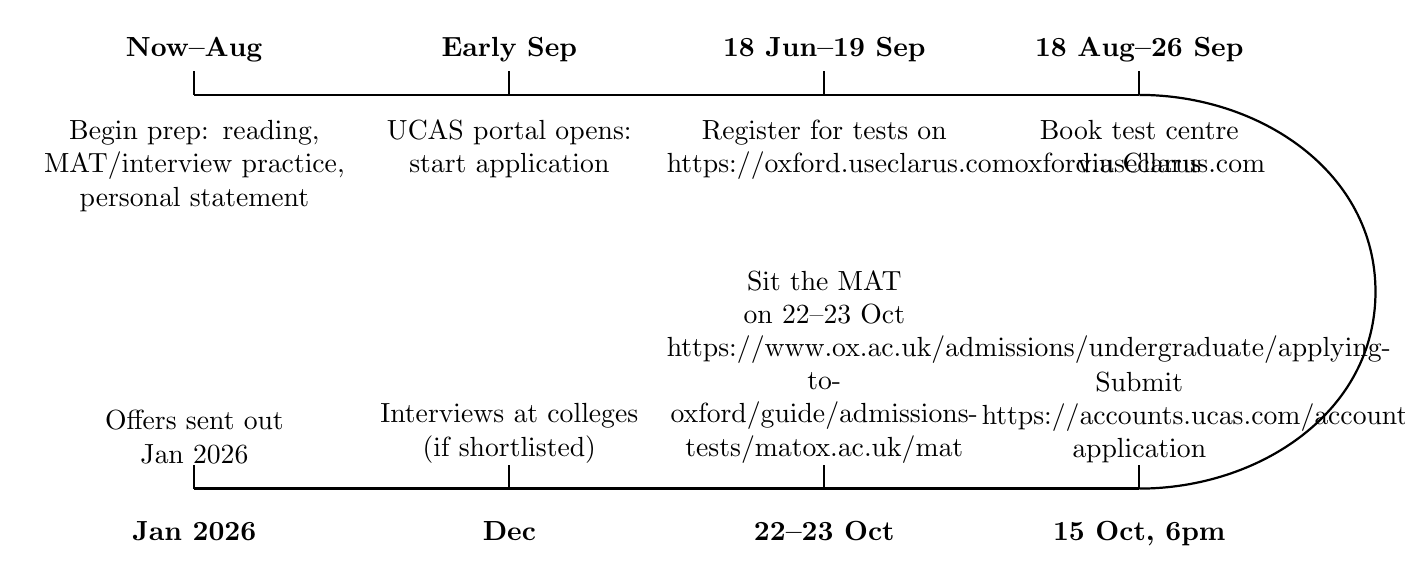
\begin{tikzpicture}[>=Stealth]
\usetikzlibrary{calc}
% --- Top row (left to right) ---
\coordinate (prep)      at (0,0);
\coordinate (ucasopen)  at (4,0);
\coordinate (clarus)    at (8,0);
\coordinate (booking)   at (12,0);

% --- Downward turn ---
\coordinate (turn)      at (15,-2.5);

% --- Bottom row (right to left) ---
\coordinate (ucasclose) at (12,-5);
\coordinate (matdates)  at (8,-5);
\coordinate (interviews)at (4,-5);
\coordinate (offers)    at (0,-5);

% --- Draw arrows ---
\draw[thick] (prep) -- (booking);              % Top row
\draw[thick] (booking) to[out=0, in=90] (turn) to[out=270,in=0] (ucasclose);
\draw[thick] (ucasclose) -- (offers);               % Bottom row

% --- Tick marks ---
\foreach \pt in {prep, ucasopen, clarus, booking, ucasclose, matdates, interviews, offers}
  \draw[thick] (\pt) -- ++(0,0.3);

% --- Dates above ---
\node[align=center, anchor=south] at ($(prep)+(0,0.3)$) {\textbf{Now–Aug}};
\node[align=center, anchor=south] at ($(ucasopen)+(0,0.3)$) {\textbf{Early Sep}};
\node[align=center, anchor=south] at ($(clarus)+(0,0.3)$) {\textbf{18 Jun–19 Sep}};
\node[align=center, anchor=south] at ($(booking)+(0,0.3)$) {\textbf{18 Aug–26 Sep}};

\node[align=center, anchor=north] at ($(ucasclose)-(0,0.3)$) {\textbf{15 Oct, 6pm}};
\node[align=center, anchor=north] at ($(matdates)-(0,0.3)$) {\textbf{22–23 Oct}};
\node[align=center, anchor=north] at ($(interviews)-(0,0.3)$) {\textbf{Dec}};
\node[align=center, anchor=north] at ($(offers)-(0,0.3)$) {\textbf{Jan 2026}};

% --- Descriptions below/above ---
\node[align=center, anchor=north, text width=4cm] at ($(prep)-(0,0.2)$) {
Begin prep: reading,\\MAT/interview practice,\\personal statement
};
\node[align=center, anchor=north, text width=4cm] at ($(ucasopen)-(0,0.2)$) {
UCAS portal opens:\\start application
};
\node[align=center, anchor=north, text width=4cm] at ($(clarus)-(0,0.2)$) {
Register for tests on\\\href{https://oxford.useclarus.com}{oxford.useclarus.com}
};
\node[align=center, anchor=north, text width=4cm] at ($(booking)-(0,0.2)$) {
Book test centre\\via Clarus
};

\node[align=center, anchor=south, text width=4cm] at ($(ucasclose)+(0,0.2)$) {
	Submit \href{https://accounts.ucas.com/account/login}{UCAS}\\application
};
\node[align=center, anchor=south, text width=4cm] at ($(matdates)+(0,0.2)$) {
Sit the MAT on 22–23 Oct\\\href{https://www.ox.ac.uk/admissions/undergraduate/applying-to-oxford/guide/admissions-tests/mat}{ox.ac.uk/mat}
};
\node[align=center, anchor=south, text width=4cm] at ($(interviews)+(0,0.2)$) {
Interviews at colleges\\(if shortlisted)
};
\node[align=center, anchor=south, text width=4cm] at ($(offers)+(0,0.2)$) {
Offers sent out\\ Jan 2026
};

\end{tikzpicture}
}
\end{center}
%--------------------------------------------------


\subsection{UCAS application}

This involves the personal statement and other things you have little control over (such as previous academic record and teacher reference).  For Maths at good universities like Cambridge and Oxford, your personal statement is largely irrelevant. This is because they have better means to measure the suitability of a
candidate for their course, such as interviews and admissions tests.

What you should take away from this isn’t that you don’t need to write a good personal statement, but that
you don’t need to worry about doing extremely specific extracurriculars or very minute details. Make sure the statement is good for other universities. They’re generally not interested at all in anything in your personal statement that isn’t about maths, but
it is good to have a line or two on this for the sake of other universities. In the interview, they’re generally
unlikely to ask you about anything in your personal statement, but you should be aware of what you wrote. 

Doing extracurricular maths shouldn't be done for the sake of including it in the personal statement, but because it will be really good preparation for university. To this end, the wider reading books I've included and the MOOCs are probably especially helpful. 

\href{https://www.undergraduate.study.cam.ac.uk/apply/how/ucas-personal-statement}{Advice from Cambridge} on personal statements. 

\href{https://www.ox.ac.uk/admissions/undergraduate/applying-to-oxford/guide/ucas-application}{Advice from Oxford} on personal statements.

\subsection{Admissions tests}

For Oxford, you have to sit the \href{https://www.maths.ox.ac.uk/study-here/undergraduate-study/maths-admissions-test}{MAT}. This is a \textbf{major} factor in determining whether to invite you for an interview, and also plays a role in the final decision after the interview, so it is important to do well. 50\% is probably enough to get invited for an interview, but 75\% is the average for accepted applicants --- as mentioned previously, it is probably best to aim for 90\%+. 

For Cambridge, you have to sit \href{https://www.maths.cam.ac.uk/undergrad/admissions/step}{STEP}, which is done in the summer and constitutes part of the conditional offer. It is thus much harder, as you will have covered all of the A-level content by this point.  

The best way to prepare for both of these exams is to do maths questions. Lots of them! This will involve past paper questions as well as lots of others. If you ever need a break from doing questions, then maybe read the technical books I've included as well.


\subsection{Interviews}

The interview is not something to worry about --- in fact, you will do better if you don't! You will probably have multiple interviews at multiple colleges. The interviews are almost entirely academic, but it is always worth having an answer prepared to ‘Why do you like maths? ’ Just so you don't come across as a numpty.

\personal{I got asked this in mine! They might also ask some other ice-breaker questions just to relax you --- your answer won't affect your interview score!}

Make sure to speak aloud about what you’re thinking, which
allows them to assess you. Also, make sure you listen carefully to what the interviewers
say. It’s ok to be silent for a bit if you need to think, and it’s ok to get something wrong; the interviewers will help push you in the right direction to solve the problem. 

They want to see how you think, so in essence, the interview only starts when you no longer know the answer straight away! This is how they assess your potential for learning from the tutorial system in Oxbridge.  Since this is probably the most novel part of the whole application process, I’d strongly encourage you to ask teachers or mentors for mock interviews and to practise talking through your reasoning aloud. It is also very useful to go on YouTube and search for recordings of past interviews, for example \href{https://www.youtube.com/watch?v=lcFMcohMcVQ}{here}. I've also included some sample interview questions below.

\comment{You are already very good at talking through your thinking, so just keep doing what you're doing!}

There is also more information about interviews produced by Oxford \href{https://www.ox.ac.uk/admissions/undergraduate/applying-to-oxford/guide/interviews}{here}.

\section{Resources}

This is by no means a complete list — rather, it’s a collection of things I did which I found interesting or useful in some way. If you'd like more details on any of the sections, feel free to ask. The order is not significant — in fact, you might find some of the later items the most enjoyable or valuable.

\subsection{Exam Practice}

\begin{enumerate}
\item \href{https://www.maths.ox.ac.uk/study-here/undergraduate-study/maths-admissions-test}{MAT past papers}. While the syllabus and format have changed recently, the old papers remain an excellent source of problems and give you the clearest idea of what to expect. I’d recommend starting with the earlier ones and working your way forward.

\item \href{https://www.colmanweb.co.uk/Assets/PDF/advanced-problems-mathematics.pdf}{Stephen Siklos' STEP Book}. STEP past paper questions are also brilliant practice, though they can be very challenging at first. That’s why this book is helpful — it includes worked solutions and helps bridge the gap into STEP-style thinking.


\item \href{https://maths.org/step/assignments-stepiii}{\textbf{Step practice modules}} these are produced by Cambridge University and exist for STEP I, II, and III and are nice and accessible.
\end{enumerate}

\subsection{Sample interview questions}

\begin{itemize}

\item \href{https://www.drfrost.org/uploads/users/1/r261/TBO\%20Problem\%20Solving\%20Booklet.pdf}{\textbf{TBO Problem Solving Booklet}} --- some very good problems in the style of interview questions. 

\item \href{https://vg354.user.srcf.net/resources/Interview_questions.pdf}{\textbf{Example interview questions}} --- some more past interview questions.

\item \href{https://www.cl.cam.ac.uk/\string~abr28/prob/questions.pdf}{\textbf{Probability interview questions}} --- by the creator of the CSAT, some hard probability interview style questions.

\end{itemize}

\subsection{Books}

These are a selection of more technical books, wider reading is also encouraged in an effort to build a broader interest around the subject - suggestions for this are included in \cref{sec:morebooks}.

\begin{itemize}
\item \textbf{What Is Mathematics?} by Richard Courant and Herbert Robbins — a classic text that presents “older” mathematical ideas in a very elegant way. \emph{Let me know if you’d like a PDF copy.}

\item \href{https://ukmt.org.uk/product/a-problem-solvers-handbook}{\textbf{UKMT Problem Solver’s Handbook}} — one of a wider series of books from UKMT. This contains clear explanations and rich problems. \emph{I think I may have even started with the junior-level book (ages 11–13) when I was 16, since I hadn’t encountered much of this style before.}

\item \href{https://isaacphysics.org/books/pre_uni_maths_2e}{\textbf{101 Integrals}} — not a bad book overall, but the highlight is the appendix of 101 integrals. If you work through and understand these, I suspect you won’t struggle with a single A-level integral again. \emph{I used to do these during my regular maths lessons.}
  
\item \href{https://www.risps.co.uk/}{\textbf{RISPS}} — a collection of 40 mathematical investigations aimed at A-level students. Some are genuinely fascinating. There's also a companion set for Further Maths students. These are well worth exploring.
  

\item \href{https://www2.math.upenn.edu/~wilf/gfologyLinked2.pdf}{\textbf{Generatingfunctionology}} by Herbert Wilf — a book I discovered through the Penn course. I never finished it, but I found the parts I read both engaging and clearly written.
\end{itemize}

\subsection{MOOCs}

Many universities publish their entire courses online --- and you'll likely be surprised by how accessible you find them.

\personal{Over the summers of Year 11 and Year 12 (and into Year 13), I worked through the following three. I completed most of the material, and this gave me a real head start at university — I felt much more comfortable with many concepts than my peers.}

\begin{enumerate}
\item \href{https://www.coursera.org/learn/single-variable-calculus}{University of Pennsylvania: Single-Variable Calculus}. This course has beautifully animated videos and offers a thorough, enriching take on A-level content. If you do only one, make it this.

\item \href{https://ocw.mit.edu/courses/18-01-calculus-i-single-variable-calculus-fall-2020/}{MIT: Single-Variable Calculus}. This overlaps heavily with the Penn course, but it's still worth doing — seeing similar content presented in different ways helps reinforce it. Plus, the exercises are different.

\item \href{https://ocw.mit.edu/courses/18-02-multivariable-calculus-fall-2007/}{MIT: Multivariable Calculus}. This is where I really learned multivariable calculus — and, perhaps tellingly, it's still the way I think about it, despite having taken the course formally at Oxford.
\end{enumerate}


\subsection{UKMT \& Olympiads}

There are many mathematical Olympiads that happen, including most famously the \href{https://www.imo-official.org/}{IMO (International Mathematical Olympiad)}. The \href{https://ukmt.org.uk/}{\textbf{UKMT}} — they run the Senior Maths Challenge and the British Mathematical Olympiad (BMO). A good target is to get a Merit in BMO Round 1 — that puts you roughly in the top 400 in your age group. Oxford and Cambridge together admit about that many maths students per year. \personal{That said, most people I knew who applied had simply achieved a high-scoring Gold in the Senior Maths Challenge (the round before the Olympiad).}

\section{Next steps}

Start by looking through the above resources and finding ones you enjoy. Maths books are best read slowly with lots of repetition. Do problems as and when you can. Try to find stuff that interests you. 

\personal{While I’ve tried to present this as objectively as possible, bear in mind that it’s all based on my experience. A love of the subject will get you much, much further (eventually) than any kind of natural talent or ability.}


\appendix

\section{More wider reading}\label{sec:morebooks}

\personal{I think I might have flicked through a couple of these, but I don't think I seriously read any of them, so can't comment on how good they are!}

\begin{itemize}

\item \href{https://isbn.is/9780297819929}{\textbf{The Magical Maze}} — Structured around the image of a maze representing interconnected mathematical ideas. Covers numbers, probability, game theory, patterns, oscillators, knots, computability, chaos, and more.

\item \href{https://isbn.is/9781846680649}{\textbf{Cabinet of Mathematical Curiosities}} — Hidden gems in logic, geometry, and probability. Includes puzzles like extracting cherries from cocktail glasses, a pop-up dodecahedron, and insights into familiar names like Pythagoras and prime numbers.

\item \href{https://isbn.is/9780747597162}{\textbf{Alex's Adventures in Numberland}} — Explores the geometry of the 50p coin, gambling strategies, mathematical patterns in nature, and the peculiar predictability of randomness.

\item \href{https://isbn.is/9781402757969}{\textbf{The Math Book}} — A historical tour through 250 short entries on major theorems and the mathematicians who discovered them. By Clifford Pickover.

\item \href{https://isbn.is/014017480X}{\textbf{You Are a Mathematician}} — Begins with the familiar and journeys through mathematical history from the Greeks to quantum theory. By David Wells.

\item \href{https://isbn.is/1862075557}{\textbf{It Must Be Beautiful}} — An accessible exploration of great equations of modern science, presented for non-specialists by various authors.

\item \href{https://isbn.is/1841155802}{\textbf{The Music of the Primes}} — A deep dive into the Riemann hypothesis and the hidden pattern of prime numbers. By Marcus du Sautoy.

\item \href{https://isbn.is/9780007214624}{\textbf{Finding Moonshine}} — A book full of insight into the nature of symmetry and the lives of those who study it. By Marcus du Sautoy.

\item \href{https://isbn.is/0691095418}{\textbf{Trigonometric Delights}} — An entertaining and historical exploration of trigonometry, blending biography and mathematics. By Eli Maor.

\item \href{https://isbn.is/9780385415804}{\textbf{The Prisoner's Dilemma}} — Explains game theory with clarity and brings the story of John von Neumann to life. By William Poundstone.

\item \href{https://isbn.is/0333780337}{\textbf{E = mc²}} — A biography of the world's most famous equation. By David Bodanis.

\item \href{https://isbn.is/9780140147391}{\textbf{Journey Through Genius}} — Explores some of the most profound theorems of mathematics and the stories behind them. By William Dunham.

\item \href{https://isbn.is/1862077355}{\textbf{The Millennium Problems}} — The seven greatest unsolved mathematical problems of our time. By Keith Devlin.

\item \href{https://isbn.is/0571212921}{\textbf{A Beautiful Mind}} — The life of Nobel laureate and mathematical genius John Nash. By Sylvia Nasar.

\item \href{https://isbn.is/0749386061}{\textbf{Chaos}} — A classic introduction to the science of chaos and unpredictability. By James Gleick.

\item \href{https://isbn.is/0140144110}{\textbf{Fractal: Images of Chaos}} — A visual exploration of fractals in computer art, population models, and planetary motion. By Hans Lauwerier.

\item \href{https://isbn.is/9780140276664}{\textbf{Six Easy Pieces}} — Richard Feynman’s clear explanation of fundamental physics concepts.

\item \href{https://isbn.is/0099736217}{\textbf{Feynman's Lost Lecture}} — A beautiful and accessible explanation of planetary motion. By David and Ruth Goodstein.

\item \href{https://isbn.is/0906212898}{\textbf{Images of Infinity}} — A creative mix of images, writings, and paradoxes related to infinity. Published by Tarquin Press.

\item \href{https://isbn.is/0883857006}{\textbf{Proofs Without Words (Book 1)}} — Visual demonstrations of mathematical truths. By Roger B. Nelson.

\item \href{https://isbn.is/0883857219}{\textbf{Proofs Without Words (Book 2)}} — A second volume of beautifully illustrated visual proofs. By Roger B. Nelson.

\item \href{https://isbn.is/1841157910}{\textbf{Fermat’s Last Theorem}} — The dramatic story of the 350-year mystery finally solved by Andrew Wiles. By Simon Singh.

\item \href{https://isbn.is/1857028899}{\textbf{The Code Book}} — The history of cryptography from the ancient world to modern-day ciphers. By Simon Singh.

\item \href{https://isbn.is/000717604X}{\textbf{The Cracking Code Book}} — A practical and engaging introduction to breaking codes. By Simon Singh.

\item \href{https://isbn.is/0140256024}{\textbf{Does God Play Dice?}} — An excellent introduction to chaos theory. The title quotes Einstein’s skepticism. By Ian Stewart.

\item \href{https://isbn.is/0140132376}{\textbf{Game, Set and Math}} — Mathematical insights into tennis, puzzles, and beyond. By Ian Stewart.

\item \href{https://isbn.is/0007214227}{\textbf{Longitude}} — The true story of the quest to solve the longitude problem at sea. By Dava Sobel.

\item \textbf{Mathematical Puzzles and Diversions}, \textbf{More Mathematical Puzzles and Diversions}, \textbf{Mathematical Circus}, \textbf{The Unexpected Hanging}, \textbf{Fractal Music, Hypercards and More} — All by Martin Gardner. A treasure trove of mathematical amusement and insight.

\item \href{http://www.geom.uiuc.edu/~banchoff/Flatland/}{\textbf{Flatland – A Romance of Many Dimensions}} — A story of a square living in a two-dimensional world and his encounter with a sphere. By Edwin A. Abbott. Also available to read online.

\end{itemize}

\appendix
\section{Exam Technique and Strategy for STEP and MAT}\label{sec:examtips}

\subsection{Exam Technique}
\begin{itemize}
\item (\textbf{STEP and MAT}) Spend 5--10 minutes at the start selecting which questions to attempt. For STEP, it's better to do several almost-complete solutions than many partial ones. For MAT, skim through all questions to spot the accessible multiple-choice items and quickly mark any you can solve instantly.
\item (\textbf{STEP}) Very little credit is given for only completing the first part of a question. Focus on complete or nearly complete solutions.
\item (\textbf{STEP}) Longer questions with many parts may be easier. Favour questions with step-by-step guidance.
\item (\textbf{STEP and MAT}) Choose questions where the next step is relatively clear. Look for those offering structured prompts.
\item (\textbf{STEP}) 5--6 good but incomplete solutions can earn a grade 1, but aim for at least 2--3 fully complete ones.
\item (\textbf{STEP}) Prefer questions that say \textquotedblleft show that...\textquotedblright\ as they guide you more clearly and may offer partial credit for progress.
\item (\textbf{STEP}) Seek questions with accessible marks, e.g., those requiring simple differentiation, even if the final result is difficult.
\item (\textbf{STEP}) Don't rely on fragmentary attempts. You need at least 5 questions with a solid number of attainable marks.
\item (\textbf{STEP}) Be wary of questions requiring clever substitutions unless you can immediately see the approach.
\item (\textbf{STEP}) If stuck after 30--40 minutes, write what you'd do next to earn method marks before moving on.
\item (\textbf{STEP}) Question 1 is often the most accessible, followed by Question 2.
\item (\textbf{MAT}) For multiple choice, eliminate clearly wrong answers first. Use estimation, graph behaviour, and logical reasoning if you can’t compute an answer directly.
\item (\textbf{MAT}) Time management is crucial. Don’t spend too long on one problem; flag hard ones and revisit if time allows.
\end{itemize}

\subsection{Using Earlier Parts to Help with Later Parts (STEP only)}
\begin{itemize}
\item Substitutions often transform later parts into versions of earlier parts.
\item Sometimes, methods used earlier need to be adapted for later parts.
\item Calculated values in early parts might reveal patterns or help deduce later results.
\item Similar equations often appear with slight variations --- spot and reuse prior work.
\item If the second part looks different, it may just require substitution from the first part.
\end{itemize}

\subsection{Approaches}
\begin{itemize}
\item (\textbf{STEP}) Earlier parts almost always help with later parts --- use \textquotedblleft hence\textquotedblright\ when given.
\item (\textbf{STEP}) "Deduce" usually implies a short logical step, but rigour is still needed.
\item (\textbf{STEP}) Modify given substitutions when no guidance is provided in later parts.
\item (\textbf{STEP and MAT}) Factorisation helps determine sign and structure, especially with primes/integers.
\item (\textbf{STEP and MAT}) Don't overthink the stem or early parts --- they're usually approachable.
\item (\textbf{STEP and MAT}) If algebra looks messy, seek a faster route or simplification.
\item (\textbf{STEP and MAT}) Always check and justify any constraints (e.g. \$|x|<1\$) before applying results.
\end{itemize}

\subsection{Sequences, Series and Recurrences (mainly STEP)}
\begin{itemize}
\item Look at initial terms to spot a pattern; prove it by induction.
\item If unsure of the pattern, consider how the sequence is generated.
\item Use method of differences where possible (e.g., with logs).
\item Justify convergence in infinite series before cancelling.
\item For series with terms like $2^{-n}$, a suitable value of \$x\$ often simplifies the sum.
\end{itemize}

\subsection{Recurrence Integrals (STEP only)}
\begin{itemize}
\item \textbf{Approach 1}: Use integration by parts on $I_n$ or $I_{n+1}$.
\item \textbf{Approach 2}: Combine $I_n$ and $I_{n+1}$ using common denominators to simplify.
\item Example:
\begin{align*}
I_n + I_{n+1} &= \int_0^1 \frac{1}{(1+x)^n} , dx + \int_0^1 \frac{1}{(1+x)^{n+1}} , dx \\
&= \int_0^1 \frac{1+x}{(1+x)^{n+1}} , dx + \int_0^1 \frac{1}{(1+x)^{n+1}} , dx \\
&= \int_0^1 \frac{2+x}{(1+x)^{n+1}} , dx
\end{align*}
\end{itemize}

\subsection{Graphs (STEP and MAT)}
\begin{itemize}
\item Determine domain (where the function is defined).
\item Examine behaviour as $x \to \pm\infty$ and near asymptotes.
\item Identify $x$- and $y$-intercepts.
\item Find turning/inflection points if needed. Use differentiation only if necessary.
\item Check vertical scale with specific points.
\item Similar-looking graphs in the same question may be transformations.
\end{itemize}

\subsection{Algebra (STEP and MAT)}
\begin{itemize}
\item Multivariable polynomials can often be factorised similarly to single-variable ones:
\begin{align*}
x^3 - 4x^2y - xy^2 + 4y^3 = (x - y)(x - 4y)(x + y)
\end{align*}
\item For modulus functions, split into cases based on $x$.
\item When finding extrema on intervals, test endpoints and turning points.
\item If algebra looks long-winded, look for substitutions or structure.
\item Example:
\begin{align*}
x^2 - 4x + \sqrt{2x^2 - 8x - 3} - 9 = 0 \\
\text{Let } y = \sqrt{2x^2 - 8x - 3}, \text{ then use } x^2 - 4x = \tfrac{1}{2}(y^2 + 3)
\end{align*}
\item For large numbers, factor them to simplify.
\item Use coefficient comparison when working with identities.
\item Remember $\sqrt{x^2} = |x|$, not $x$.
\item Polynomial root results may appear in geometry problems.
\item If a solution becomes undefined, consider limits or alternate forms.
\item Always simplify algebra in mechanics to reduce error risk.
\item Look for symmetry --- if $a + b - c$ is a factor and the expression is symmetric, so are the cyclic variants.
\end{itemize}



\end{document}

